\documentclass{article}
\usepackage{float}
\usepackage{graphicx}
\usepackage{amsmath}
\usepackage{listings}
\usepackage{color}
\usepackage{multicol}
\usepackage{cancel}
\definecolor{cadmiumgreen}{rgb}{0.0, 0.42, 0.24}
\lstset{frame=tb,
  language=R,
  aboveskip=3mm,
  belowskip=3mm,
  showstringspaces=false,
  columns=flexible,
  basicstyle={\small\ttfamily},
  numbers=none,
  numberstyle=\tiny\color{gray},
  keywordstyle=\color{blue},
  commentstyle=\color{dkgreen},
  stringstyle=\color{cadmiumgreen},
  breaklines=true,
  breakatwhitespace=true,
  tabsize=3
}
\usepackage[margin=0.75in]{geometry}
\setlength\parindent{0pt}

\title{Seismo 512 HW 5}
\date{2/06/2023}
\author{Simon-Hans Edasi}

\begin{document}

	\maketitle

%%%%%%%%%%%%%%%%%%%%%%%%%%%%%%%%%%%%%%%%%%%%%%%%%%
\section{}

\begin{figure}[H]
    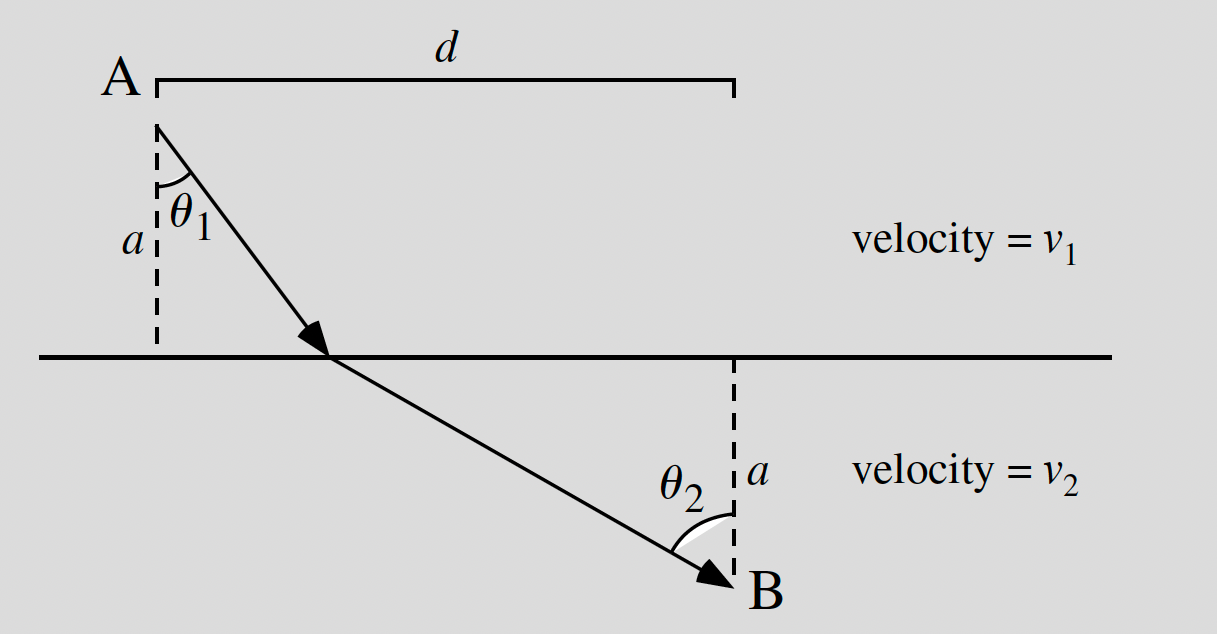
\includegraphics[scale = 0.17]{snell__exercise_4.3.png}
\end{figure}
(8 points) Show that the minimum time path between points A and B for the ray geometry in Figure 4.26 gives the same result as Snell’s law.\\
(Hint: what is the total travel time of the ray in this configuration as a function of distances and velocities?)\\

\textbf{Snell's Law}: $\frac{\sin{\theta_{1}}} {V_{1}} = \frac{\sin{\theta_{2}}}{V_{2}}$. Let the base of the triangle of $\theta_{1}$ be $x$ and the base of the triangle of $\theta_{2}$ be $(d-x)$.\\

Travel time $t = \frac{distance}{velocity}$ 


\[
t = \frac{\sqrt{a^{2}+x^{2}}}{V_{1}} + \frac{\sqrt{a^{2}+\left(d-x\right)^{2}}}{V_{2}}
\]
A minimum time path between points means $\frac{dt}{dx} = 0$, so:

\[
\frac{dt}{dx} = V_{1}^{-1} \frac{1}{\bcancel{2}}\bcancel{2}x\left(a^{2} + x^{2}\right)^{-\frac{1}{2}} + V_{2}^{-1}\frac{1}{\bcancel{2}}\bcancel{2}\left(d-x\right)\left(a^{2} + \left(d-x\right)^{2}\right)^{-\frac{1}{2}} = 0
\]

\[
\frac{x}{V_{1}\sqrt{a^{2}+x^{2}}} - \frac{d-x}{V_{2}\sqrt{a^{2}+\left(d-x\right)^2}} = 0 \quad\rightarrow\quad \frac{x}{V_{1}\sqrt{a^{2}+x^{2}}} = \frac{d-x}{V_{2}\sqrt{a^{2}+\left(d-x\right)^2}}
\]

$\frac{x}{\sqrt{a^{2}+x^{2}}} = \sin{\theta_{1}}$ and $\frac{d-x}{\sqrt{a^{2}+\left(d-x\right)^2}} = \sin{\theta_{2}}$\\

QED 














\end{document}
